\documentclass[tikz,border=2pt]{standalone}
\usepackage{amsmath}
\usetikzlibrary{arrows.meta}
\begin{document}
% Dutch auction as a clock: the price falls from 1; bidder 1 (theta_1 = 0.8) plans to stop at
% b_1 = theta_1/2 = 0.4, bidder 2 at b_2 = theta_2/2 < 0.4. The clock reaches 0.4 first, so bidder 1
% wins and pays 0.4: the highest planned stopping price wins and is paid, as in a first-price auction.
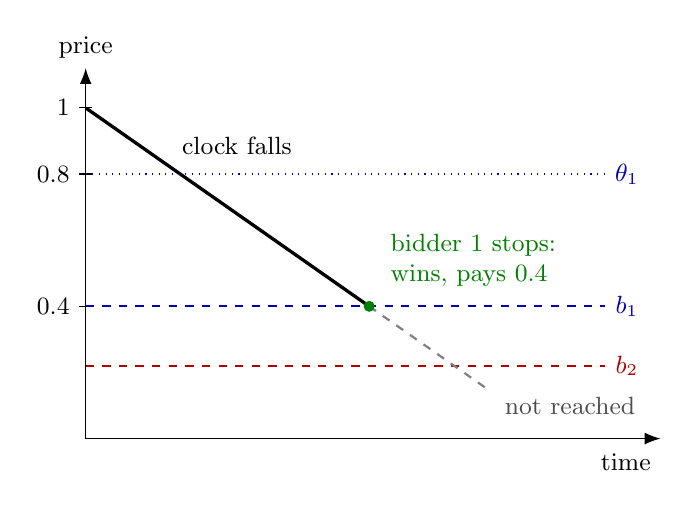
\begin{tikzpicture}[font=\small, >={Latex[length=2mm]}, x=1cm, y=4.2cm]
  % axes
  \draw[->] (0,0) -- (7.3,0) node[anchor=north east, yshift=-2pt] {time};
  \draw[->] (0,0) -- (0,1.12) node[anchor=south] {price};
  \foreach \p/\l in {1/$1$, 0.8/$0.8$, 0.4/$0.4$}
    \draw (0.08,\p) -- (-0.08,\p) node[anchor=east] {\l};
  % value of bidder 1
  \draw[blue!70!black, thin, dotted] (0,0.8) -- (6.6,0.8) node[anchor=west] {$\theta_1$};
  % planned stopping prices
  \draw[blue!70!black, thick, dashed] (0,0.4) -- (6.6,0.4) node[anchor=west] {$b_1$};
  \draw[red!70!black, thick, dashed] (0,0.22) -- (6.6,0.22) node[anchor=west] {$b_2$};
  % clock path: falls from 1 until it hits b_1
  \draw[gray, thick, dashed] (3.6,0.4) -- (5.1,0.15);
  \draw[very thick] (0,1) -- (3.6,0.4);
  \fill[green!50!black] (3.6,0.4) circle (2pt);
  \node[green!50!black, anchor=south west, align=left] at (3.75,0.43) {bidder 1 stops:\\ wins, pays $0.4$};
  \node[gray!60!black, anchor=west] at (5.2,0.1) {not reached};
  \node[anchor=south west] at (1.1,0.83) {clock falls};
\end{tikzpicture}
\end{document}
